%!TEX root = gorila_paper.tex
\subsection{Reinforcement Learning}

\begin{figure}[ht]
    %\vskip -0.1in
    \begin{center}
        \centerline{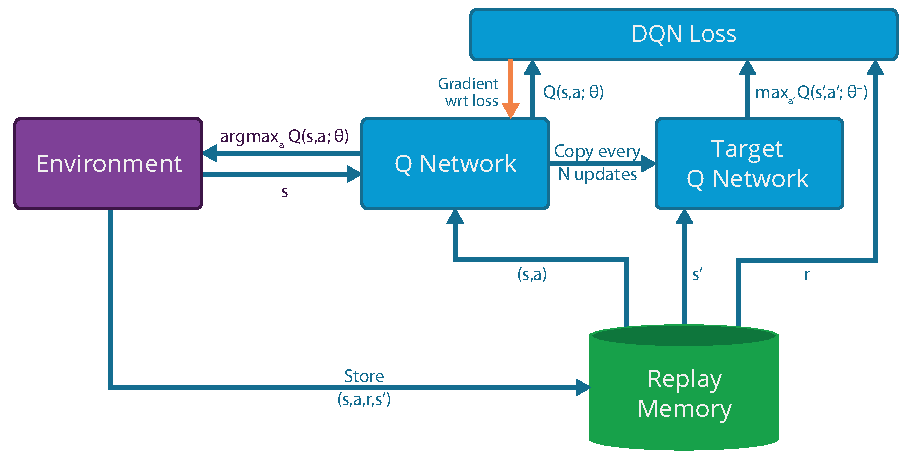
\includegraphics[width=\columnwidth]{DQNAgent_1}}
        \caption{The DQN algorithm is composed of three main components, the Q-network $(Q(s,a;\theta))$ that defines the behavior policy, the target Q-network $(Q(s,a;\theta^-))$ that is used to generate target Q values for the DQN loss term and the replay memory that the agent uses to sample random transitions for training the Q-network.}
        \label{DQN-figure}
    \end{center}
    \vskip -0.2in
\end{figure}

In the reinforcement learning (RL) paradigm, the agent interacts sequentially with an environment, with the goal of maximising cumulative rewards. At each step $t$ the agent observes state $s_t$, selects an action $a_t$, and receives a reward $r_t$. The agent's \emph{policy} $\pi(a | s)$ maps states to actions and defines its behavior. The goal of an RL agent is to maximize its expected total reward, where the rewards are discounted by a factor $\gamma \in [0,1]$ per time-step. Specifically, the \emph{return} at time $t$ is $R_t =\sum\limits_{t'=t}^{T} \gamma^{t'-t}r_{t'}$  where $T$ is the step when the episode terminates. The \emph{action-value function} $Q^\pi(s,a)$ is the expected return after observing state $s_t$ and taking an action under $a$ policy $\pi$, $Q^\pi(s,a) = \expect{}{R_t | s_t=s, a_t=a, \pi}$, and the \emph{optimal} action-value function is the maximum possible value that can be achieved by any policy, $Q^*(s,a) = \argmax{\pi}{Q^\pi(s,a)}$. The action-value function obeys a fundamental recursion known as the Bellman equation, $Q^*(s,a) = \expect{}{r + \gamma \ \max{a'}{Q^*(s',a')}}$. 

One of the core ideas behind reinforcement learning is to represent the action-value function using a function approximator such as a neural network, $Q(s,a) = Q(s,a; \theta)$. The parameters $\theta$ of the so-called \emph{Q-network} are optimized so as to approximately solve the Bellman equation. For example, the Q-learning algorithm iteratively updates the action-value function $Q(s,a; \theta)$ towards a sample of the Bellman target, $r + \gamma \ \max{a'}{Q(s',a'; \theta)}$. However, it is well-known that the Q-learning algorithm is highly unstable when combined with non-linear function approximators such as deep neural networks~\cite{tsitsiklis-convergence}. 

\subsection{Deep Q-Networks}
Recently, a new RL algorithm has been developed which is in practice much more stable when combined with deep Q-networks \cite{mnih2013atari,mnih-dqn-2015}. Like Q-learning, it iteratively solves the Bellman equation by adjusting the parameters of the Q-network towards the Bellman target. However, DQN, as shown in Figure~\ref{DQN-figure} differs from Q-learning in two ways. First, DQN uses experience replay \cite{lin1993reinforcement}. At each time-step $t$ during an agent's interaction with the environment it stores the experience tuple $e_t = (s_t, a_t, r_t, s_{t+1})$ into a replay memory $D_t = \{e_1, ..., e_t\}$. 

Second, DQN maintains two separate Q-networks $Q(s,a; \theta)$ and $Q(s,a; \theta^-)$ with current parameters $\theta$ and old parameters $\theta^-$ respectively. The current parameters $\theta$ may be updated many times per time-step, and are copied into the old parameters $\theta^-$ after $N$ iterations. At every update iteration $i$ the current parameters $\theta$ are updated so as to minimise the mean-squared Bellman error with respect to old parameters $\theta^-$, by optimizing the following loss function (DQN Loss),
%
\begin{small}
\begin{align}
L_i(\theta_i) = \expect{}{\left( r + \gamma \ \max{a'} Q(s', a'; \theta_i^-) - Q(s, a; \theta_i) \right)^2}
\end{align}
\end{small}
%
For each update $i$, a tuple of experience $(s,a,r,s') \sim U(D)$ (or a minibatch of such samples) is sampled uniformly from the replay memory $D$. For each sample (or minibatch), the current parameters $\theta$ are updated by a stochastic gradient descent algorithm. Specifically, $\theta$ is adjusted in the direction of the sample gradient $g_i$ of the loss with respect to $\theta$,
%
\begin{small}
\begin{align}
g_i = \left( r + \gamma \ \max{a'} Q(s', a'; \theta_i^-) - Q(s, a; \theta_i) \right) \nabla_{\theta_i} Q(s,a; \theta)
\label{eqn:dqngrad}
\end{align}
\end{small}
%
Finally, actions are selected at each time-step $t$ by an $\epsilon$-greedy behavior with respect to the current Q-network $Q(s,a;\theta)$.
